\chapter{Decoding with Ordinal Labels}\label{chap:decoding_ordinal}
\markright{{~{\rm \ref{chap:decoding_ordinal}}. Decoding with Ordinal Labels}\hfill}{}


\vspace*{\fill}
\newthought{We have presented} in Chapter 2 the decoding problem in fMRI. In this setting it is often the case that the target variable consists of discretely ordered values. This occurs for example when target values consists of human generated ratings, such as values on a Likert scale, the symptoms of a physical disease or a rating scale for clinical pain measurement.

In this chapter we propose the usage of two metrics to assess the performance of a decoding model when the target consists of discretely ordered values: the absolute error and pairwise disagreement. These two loss functions emphasize different aspects of the problem: while the absolute error gives a measure of the closeness of a predicted label to the true label, the pairwise disagreement gives a measure of correct ordering of the predicted labels. The choice of either metric will depend on the particular application at hand. For example, in clinical applications it is often desirable to predict a label as close as possible to the true label, in which case the absolute error is the appropriate metric. If however, the purpose of the decoding study is to perform a statistical hypothesis test to claim that the area encodes some information about the stimuli, then the pairwise disagreement can be considered.


We present three models based on different convex surrogates of the absolute error: least absolute error, ordinal logistic regression and cost-sensitive multiclass classification. We also consider a model that minimizes a surrogate of the pairwise disagreement: the RankLogistic model. We examine the generalization performance of the presented models on both synthetic data and three fMRI decoding problems from two datasets. We conclude that the best performing models is the last absolute error and ordinal logistic when considering the absolute error as metric and the RankLogistic model when considering the pairwise disagreement as metric. 



%\hspace{20pt}
\begin{shaded}
The contributions relative to the use of the pairwise disagreement loss function have been published in:
\begin{itemize}
\item F. Pedregosa, E. Cauvet, G. Varoquaux, C. Pallier, B. Thirion, and A. Gramfort, \emph{``Learning to rank from medical imaging data''}, in Proceedings of the 3rd International Workshop on Machine Learning in Medical Imaging, 2012.
\end{itemize}
\end{shaded}

\newpage 
\vspace*{\fill}
\minitoc
\vspace*{\fill}
\newpage

%%%%%%%%%%%%%%%%%%%%%%%%%%%%%%%%%%%%%%%%%%%%%%
%%% Introduction
%%%%%%%%%%%%%%%%%%%%%%%%%%%%%%%%%%%%%%%%%%%%%%
%

\section{Learning from ordinal labels}

Let us motivate the problem of learning from ordinal labels by a decoding example. In the context of an fMRI acquisition, a subject is presented a set of words that represent real world objects:
hammer, cow, sheep and whale. We are then interested to know whether it is possible to predict (i.e. \emph{decode}) the implied real world size of the associated objects (i.e. the size of a goat rather than the size of the word ``goat'') based on the brain activation maps. How can we do this ?

% These stimuli cab be ordered according to their relative size. That is, the smallest animal is assigned the size 1, the next animal by size is assigned the size 2 and so on. We are now asked to predict the relative size of the animal based on the activation maps of that fMRI acquisition. 
% How can we do this ?

\begin{figure}

\includegraphics[width=\linewidth]{chapter_4/experiment.png}
\caption{In this experiment, the stimuli are words that represent real world objects. As in the Figure, these can be ordered according the the size of the associated concepts. The decoding problem will be then to predict the size of the associated concepts based on the brain activation maps.}
\end{figure}



In order to frame this problem as a \gls{decoding} problem, we must choose a metric to evaluate the quality of our prediction (i.e. a \emph{loss function}). Furthermore, as we have seen in Section~\ref{subsec:surrogate_loss_functions}, many models can be seen as the minimization of a convex surrogate of a given loss function. Thus, the chosen metric will determine which are the appropriate models to choose.



We have seen in previous chapters how the 0-1 loss can be applied to situations in which the target values consists of several categories. In this case, however, the 0-1 loss might give an overly pessimistic estimate of the performance of a classifier since it treats all misclassification errors alike. Suppose that a classifier predicts always the correct size $\pm$ 1, that is, never predicts the correct label but always predicts one of the adjacent elements in terms of size. This classifier will have the worst performance possible in terms of the 0-1 error, although we might still consider that this classifier is able predict with acceptable accuracy the size of an object.


It thus seems reasonable to choose a loss function that takes into account the distance among the labels. In this Chapter we present two metrics that fulfill this request and are adapted to the problem of supervised learning with ordinal labels. These loss functions are the \emph{absolute error} and the \emph{pairwise disagreement}. The use of the of the pairwise disagreement loss in the context of brain imaging is an original contribution first proposed in~\citep{pedregosa2012learning}.


We will describe in Section \ref{sec:or_models} three different surrogate loss functions of the absolute error and one surrogate of the pairwise disagreement. In section~\ref{section:results}, we present the performance accuracy of these models in one synthetic dataset and three fMRI datasets. {It is our intention for these results to provide guidelines on what methods are overall best suited in the context of decoding with ordered labels.}

We have motivated the decoding problem with ordinal labels from a simple fMRI experiment in which the target variable is ordered according to the size of real world objects. However, the framework presented here can be applied to any situation in which the target variable consists of \emph{discrete measures with some embedded order}. For example, this includes situations in which the target variable consists of the symptoms of a physical disease such as Alzheimer's~\citep{mueller2005ways}, pain levels~\citep{PAPR:PAPR3034} or the syntactic complexity of a phrase~\citep{pallier2011cortical} to name a few.



% {\blue Each of these metrics leads to different models. Optimizing the MSE we arrive to methods known as \emph{ordinal regression} while optimizing the pairwise error leads to \emph{pairwise ranking}. For each case, we present convex surrogates and discuss optimization strategies.} 


% One possible way to approach this \gls{decoding} problem is to treat it as a multiclass classification problem. That is, the different sizes are treated as independent and unordered labels and the multiclass model is trained using those labels. However, this treats all misclassification errors alike, while in this problem it is natural to think that misclassification of two very different sizes should be penalized more severely than misclassification of items of similar size. That is, it should not be considered the same to mistake a whale with a sheep than a cow with a sheep.


% \newglossaryentry{stochastic ordering}{name={stochastic ordering},description={A real random variable A is less than a random variable B in the if P(A>x) < P(B>x)  for all x }}


% The ordinal information can be interpreted in several ways. In a probabilistic setting, i.e., when the classifier model a certain probability distribution, the model is assumed to reflect a \emph{\gls{stochastic ordering}} on the conditional distributions $P(y \leq k | X)$~\citep{McCullagh1980, Herbrich1999Regression}. For example, the proportional odds model of \citet{McCullagh1980} assumes a probability distribution of the form
% $P(y \leq j| X=x) = \sigma(\theta_j - f(x))$
% where $\sigma$ is an appropriate \emph{link function}, such as the logistic function or the probit function.

% Another interpretation is that the mislabeling cost should depend on the distance between the prediction and the true label. This can be readily used in the empirical risk minimization setting by choosing an appropriate loss function. We will discuss two loss functions for this task: the \emph{absolute error} and the \emph{pairwise disagreement}. We will discuss the different surrogates that minimize these loss functions and examine their performance on 3 fMRI datasets.




% We will discuss two different approaches for the supervised learning problem of predicting targets with ordinal labels. The first approach that we will consider, Ordinal Regression, can be seen as a supervised learning problem where (unlike in 0-1 multiclass classification) the loss function depends on the distance between the labels. The most common loss function in this setting is the \emph{absolute error} loss function~\citep{Cardoso2011}, that we will present in Section~\ref{sec:absolute_error}. This setting includes metric regression (e.g. least absolute deviation) and multiclass formulations such as the one proposed in~\citep{lee2004multicategory} that can take into account generic losses.

% The second approach that we will consider is known as \emph{pairwise ranking}.
% Here, we do not seek to minimize the distance of a single prediction, but rather to minimize the number of inversions in an ordered list. That is, 
% given the training pairs $\{(X_1, y_1), \ldots, (X_n, y_n)\}$ so that  the sequence of training labels $\{y_1, \ldots, y_n\}$ is an ordered non-decreasing sequence, we seek to find a function $f: \XX \to \RR$ such that the sequence $\{f(X_1), f(X_2), \ldots, f(X_k)\}$ has as few inversions as possible. The loss function associated with this problem is the \emph{pairwise disagreement} that we will present in Section~\ref{sec:pairwise_disagreement}.


% Both approaches optimize different criteria and must be evaluated differently. For example, a pairwise ranking model does not output the label, thus it cannot be evaluated using the absolute error loss as an ordinal regression model. Ordinal regression models can be evaluated using the pairwise disagreement loss however.



% \subsection{Contribution}

% In this chapter we model the decoding problem in fMRI using both ordinal regression and pairwise ranking models. We present several approaches based on convex surrogates of the absolute error and pairwise disagreement loss that can be used to solve this problem. 




\section{Loss functions}\label{sec:loss_functions}

A metric that arises naturally to evaluate the quality of an ordinal prediction the distance between the predicted label $\hat{y}$ and the true label $y$, which will promote classifiers that predict a label that is close to the correct label. This is known as the \emph{absolute error} loss function, and is defined as:
\begin{equation*}
\ell_{\mathcal{A}}(y, \hat{y}) = |y - \hat{y}| 
\end{equation*}

This metric is very common when evaluating models with ordinal labels~\citep{Cardoso2011}. A related loss  worth mentioning is the squared error, often used in the regression setting. Compared to the squared error, the absolute error provides the advantage of being more robust to outliers~\citep{bloomfield1983least}.

The second loss function that we will present takes a different approach to measure the closeness of an ordinal response that does not take into account the value of the labels but rather only its relative ordering.
Unlike the absolute error loss, this loss function acts on pairs of elements. Given two elements $y_1, y_2 \in \mathcal{Y}$ and the predicted values $\hat{y}_1, \hat{y}_2 \in \RR$, this loss is defined as~\citep{schapire1998learning, Herbrich2000}:


$$
\ell_{\mathcal{P}}(y_1, y_2, \hat{y}_1, \hat{y}_1) = \mathcal{H}(- (y_1-y_2) (\hat{y}_1 - \hat{y}_2)) \quad,
$$
where we recall that $\mathcal{H}$ is the Heaviside function, defined as $\mathcal{H}(x) = 1$ if $x \geq 0$ and $0$ otherwise. That is, the loss $\ell_{\mathcal{P}}($ will be equal to one if $\hat{y}_1 - \hat{y}_2$ has not the same sign than $y_1 - y_2$ and zero otherwise. Since this loss is based on pairs of samples, the empirical risk will be evaluated on all possible pairwise combinations of elements in the training set (excluding those with same label). Given the training pairs $\{(x_1, y_1), \ldots, (x_n, y_n)\}$, the evaluation metric is defined as:
\begin{equation*}
\hat{\mathcal{R}}_{\ell_{\mathcal{P}}}(f) = \frac{1}{m} \sum_{i=1}^n \sum_{\substack{j=1\\  y_i \neq y_j}}^n \ell_{\mathcal{P}}(y_i, y_j, f(x_i), f(x_j)) \quad ,
\end{equation*}
where $m$ is the amount of pairwise combinations of samples with different labels.

% \sum_{\begin{subarray}{l} {j=1} \\ y_i \neq y_i \end{subarray}}^n \ell(y_i, y_j, f(X_i), f(X_j))


This expression can be further simplified if we consider the symmetry of the loss function. Since all pairs of labels appear twice (once for $y_i > y_j$ and once for $y_i < y_j$), we can restrict ourselves to the set of elements which verify $y_i > y_j$, in which case we can write the empirical risk as
\begin{equation}\label{eq:risk_pairwise}
\hat{\mathcal{R}}_{\ell_{\mathcal{P}}}(f) =  \frac{2}{m}\sum_{i=1}^n \sum_{\substack{j=1\\  y_i > y_j}}^n \mathcal{H}(f(x_j) - f(x_i))
\end{equation}


\section{Ranking and ordinal regression}

The different loss functions considered here lead to two different supervised learning problems. The problem in which we seek to predict an ordering as close as possible to the true ordering of a sequence of labels is traditionally known as \emph{ranking} while the problem of predicting a label as close as possible to the correct label is known as \emph{ordinal regression}.

The \emph{ordinal regression} setting was first studied by~\citep{McCullagh1980} and further developed in~\citep{Frank, Rennie, Chu2007, Keerthi2003, Chu2005a} to name a few. The minimization of the absolute error can be seen as a special case of ordinal regression. In Chapter 5 we will study ordinal regression in a general setting that includes the minimization of other loss functions such as the squared loss.

Ranking models appear chronologically later than ordinal regression. The minimization of the pairwise disagreement was proposed in~\citep{schapire1998learning} although the first attempt to minimize a convex surrogate of this loss is in
\citep{Herbrich2000}\sidenote{Although in that paper the authors refers to the proposed model (now known as RankSVM) as still as an regression models, later those same methods would be re-discovered as ranking models~\citep{Joachims2002}.}. There has been great interest in theory of ranking models in recent years with the application of these models to the field of information retrieval~\citep{Joachims2002, Burges2007, Sculley}. Analog theoretical results to the ones developed in Chapter 5 have been studied for the case of pairwise disagreement in~\citep{Duchi2006, Usunier}



% $$
% \ell_{\mathcal{P}}(\balpha, G) ~= \frac{1}{|G|}\sum_{(i \to j) \in G} \mathcal{H} (\alpha_j - \alpha_i) \quad.
% $$



% Following~\citet{Dekel2004, Duchi2006}, we present the general graph-based pairwise disagreement loss. In this setting we are given the training samples $\{X_1, \ldots, X_n\}$ and a directed acyclic graph $G$ called the \emph{preference graph}. 
% The existence of the directed edge $i \to j$ in a preference graph indicates that $i$ should be ranked higher than $j$. The goal is to produce an ordering of the training samples that is as consistent as possible with the preferences given by $G$. Given the decision function $f: \XX \to \RR$ and $\balpha = (f(x_1), \ldots, f(x_n))$, the following loss counts the number of edges that are not correctly ordered:
% $$
% \ell_{\mathcal{P}}(\balpha, G) ~= \frac{1}{|G|}\sum_{(i \to j) \in G} \mathcal{H} (\alpha_j - \alpha_i) \quad.
% $$



% We will refer to this loss as the \emph{pairwise disagreement} loss function. This generalizes the case in which the target values are of a totally ordered set, i.e., $y_1 \leq y_2 \ldots \leq y_n$, in which case the preference graph defaults to the chain.


% Note that in this case the predicted $\balpha$ has dimension $n$ (number of samples) while in the ordinal regression setting this has dimension $k$ (number of classes). This is because these two models optimize very different criteria: while the ordinal regression minimizes the \emph{pointwise} (i.e. for each sample independently) distance to the true value, the pairwise disagreement takes into account all samples and minimizes the number of pairs that do not follow the order specified by $G$. 

\section{Models}\label{sec:or_models}

The models that we present here minimize a convex surrogate of the absolute error or the pairwise disagreement loss function. We present three different surrogate loss functions for the absolute error (least absolute error, ordinal logistic regression and cost-sensitive multiclass classification) and one for the pairwise disagreement (RankLogistic). 

Because of the high dimensionality of the decoding problem and the associated risk of overfitting, the most popular choice for prediction functions in encoding and decoding models are linear decision functions~\citep{cox2003,laconte2005support, Sutao2011, thirion2006, Naselaris2011}, i.e., models in which the decision function is a linear mapping $f$ from the sample space $\mathcal{X}$ onto $\RR^d$. $d$ is an integer that depends on the model: $d=1$ in the case of least absolute error and RankLogistic, $d = k-1$ in the case of ordinal logistic regression and $d=k$ in the case of multiclass support vector machines, where $k$ is the number of classes. All models are estimated as a trade-off between a data-fitting term (the surrogate loss function) and a squared $\ell_2$ penalty that controls for overfitting. The amount of penalty is chosen by nestted cross-validation.

The training set consists of $n$ pairs $\{(\B{x}_1, y_1), \ldots, (\B{x}_n, y_n)\}$, where $\B{x}_i$ is a $p$-dimensional vector and $y_i \in [k] = \{1, 2, 'ld$.


\subsection{Least absolute error}


The first possibility that we will explore it is known as \emph{least absolute deviations}~\citep{bloomfield1980least, narula1982minimum}. We consider the following surrogate loss function $\psi_{\mathcal{A}}: \mathcal{Y} \times \RR \to \RR$:
$$
\psi_{\mathcal{A}}(y, \alpha) = |y - \alpha|  \quad.
$$

Note that this surrogate has the same expression as the absolute error $\ell_{\mathcal{A}}$. The difference strives in that the surrogates are continuous functions in their second arguments while the loss functions take values in the discrete set $[k]$. The prediction function for these surrogates is given by rounding to the closest integer in $[k]$, i.e., $\text{pred}(\alpha) = \min_{i \in [k]} |i - \alpha|$. Although this prediction rule might seem somewhat ad-hoc for the moment, we will see in the next chapter (Section~\ref{subsec:regression-based}) that it is indeed the ``optimal'' prediction function for this surrogate (in some yet to be defined notion of optimality).


The model parameters are estimated by finding the minimizer of a trade-off between a data fidelity term (the $\psi_{\mathcal{A}}$-risk) and the penalty term:


\begin{equation*}
 \quad \B{w}^*, b^* \in \argmin_{\B{w}, b} \frac{1}{n}\sum_{i=1}^n |y_i - b - \langle \B{x}_i, \B{w} \rangle|  + \lambda \|\B{w}\|^2 \quad ,
\end{equation*}


where $\B{w} \in \RR^{p}$ and $b \in \RR$ is referred to as the \emph{bias} or \emph{intercept} term. This model can be seen as a particular instance of \emph{support vector regression} with linear kernel and parameter $\varepsilon$ in the $\varepsilon$-insensitive loss set to zero. This is a well studied model for which efficient implementations have been developed~\citep{ho2012large, fan2008liblinear}. In the experiments section we will use the implementation provided in the \textrm{LIBLINEAR} library~\citep{fan2008liblinear}.

% For its widespread use we also consider the squared error loss which minimizes the \emph{sum of squares} between the true labels and the prediction 
% \begin{equation*}
% ({\bf SE}) \quad \B{w}^*, b^* \in \argmin_{\B{w}} \frac{1}{n}\sum_{i=1}^n (y_i - b - \langle \B{x}_i, \B{w} \rangle)^2  + \lambda \|\B{w}\|^2
% \end{equation*}


\subsection{Ordinal logistic regression}




% {\blue In this approach, we have seen the ordinal regression problem as a regression problem }
% This approach can be seen as the result of seeing the ordinal regression problem as a regression problem. This is called the \emph{regression-based} approach to ordinal regression.  A different model comes when you consider it as a generalization of a classification problem.

The second approach that we consider is known as \emph{ordinal logistic regression}~\citep{Rennie} and can be seen in the larger family of \emph{threshold-based ordinal regression} models~\citep{McCullagh1980,Rennie,Keerthi2003,lin2006large}. 
Let $\balpha \in \RR^{k-1}$ be the image of a decision function, that is, $\balpha = f(x)$ for some $x \in \mathcal{X}$ and consider the following prediction function:
\begin{equation}\label{eq:prediction_threshold}
\text{pred}(\balpha) = 1 + \sum_{i=1}^{k-1} \mathcal{H}(-\alpha_i) \quad .
\end{equation}

In this case, we can express the absolute error loss function in the following form:
$$
\begin{aligned}
\ell_{\mathcal{A}}(y, \hat{y}) &= |y - \left(1 + \sum_{i=1}^{k-1} \mathcal{H}(-\alpha_i)\right)| \\
&= y - 1 - \sum_{i=1}^{y-1} \mathcal{H}(-\alpha_i) + \sum_{i=y}^{k-1} \mathcal{H}(-\alpha_i)\\
&= \sum_{i=1}^{y-1} \mathcal{H}(\alpha_i) + \sum_{i=y}^{k-1} \mathcal{H}(-\alpha_i) \quad,
\end{aligned}
$$

where we have used the following property of the Heaviside function: $\mathcal{H}(x) = 1 - \mathcal{H}(-x)$.



This last formula makes it clear that the absolute error can be seen as an addition of zero-one loss functions~\sidenote{the zero-one loss can be defined in terms of the Heaviside step function as $\ell_{0-1}(y, \hat{y}) = \mathcal{H}( - y \cdot \hat{y})$.}. If we replace the Heaviside function by one of its convex surrogates such as the logistic loss, we obtain the following surrogate loss function:
\begin{equation} \label{eq:absolute_error_surrogate}
\psi_{\mathcal{M}}(y, \balpha) = \sum_{i=1}^{y-1} \varphi(-\alpha_i) + \sum_{i=y}^{k-1} \varphi(\alpha_i) \quad,
\end{equation}

where $\varphi: \RR \to \RR$ is the logistic loss, defined as $\varphi(t) = \log(1 + e^{-t})$. Note that for $k=2$, this coincides with the logistic regression model for binary 0-1 classification (Section~\ref{subsec:surrogate_loss_functions}).


When $\varphi$ is the hinge loss, this approach has been proposed under the name of \emph{Support Vector Ordinal Regression} (the implicit constraints variant)~\citep{Shashua, Chu2007}. For $\varphi$ the exponential loss, this approach was proposed by~\citep{lin2006large} as \emph{Ordinal Regression Boosting (ORBoost)}. \citet{Rennie} formulated this model for an arbitrary surrogate loss function (as it is presented here) and considered a number of surrogates, including the hinge loss and logistic loss. 
We have chosen the logistic regression as a surrogate of the 0-1 loss for ease of implementation (the surrogate is a smooth function in this case, which allows us to use gradient-based methods) rather than the more popular  \emph{Support Vector Ordinal Regression} that arises when considering the hinge loss instead. However, due to the similarity between the hinge and logistic surrogates we expect both methods to yield similar results.


% Until now we have we have considered an abstract sample space $\XX$. In the case that we are interested in, the case of decoding, each sample is a 3D image that we identify with a vector in $\RR^p$, where $p$ is the total number of voxels in the image. From now on we will denote each sample in boldface $\B{x}_i$ to emphasize that it is a vector in a $p$-dimensional space.





% For this reason, the ordinal logistic model presented here can be seen within a larger family of models known as \emph{threshold-based models} that will be considered in Chapter 5. Since the vector of thresholds partition the real line into $k$ segments, the prediction function from Eq.~\eqref{eq:prediction_threshold} can be interpreted in terms of these thresholds (Fig~\ref{fig:threshold_prediction}). Although this interpretation is not necessary to understand the results of this chapter, it is often how these models are presented within most of the literature~\citep{McCullagh1980,Rennie,Keerthi2003,lin2006large}.


In this setting we consider $\balpha$ to be of the form $\alpha_i = \theta_i - \B{x}^T \B{w}$, where $\B{w} \in \RR^p$ and $\btheta \in \RR^k$ is a non-decreasing vector known as the \emph{vector of thresholds}. 
Let us introduce the variable $s_{ij} = \sign(j - y_i + \frac{1}{2})$ for notational convenience. Then we can write the surrogate loss function from Eq.~\eqref{eq:absolute_error_surrogate} as $\sum_{i=1}^{k-1} \varphi(s_{y i} \alpha_i)$. The coefficients $\B{w} \in \RR^p$ and the vector of thresholds $\btheta = (\theta_1, \ldots, \theta_{k-1})$ will be estimated as the minimizers of the regularized empirical $\psi_{\mathcal{M}}$-risk, defined as 
\begin{equation}
\begin{aligned}
 \quad \B{w}^*, \btheta^* &\in \argmin_{\B{w}, \btheta} \frac{1}{n}\sum_{i=1}^n \left( \sum_{j=1}^{k-1} \varphi(s_{ij} (\theta_j - \langle \B{x}_i \B{w} \rangle)) \right) + \lambda \|\B{w}\|^2
\end{aligned}\label{eq:ordinal_logistic}
\end{equation}


Unlike the other models presented in this section, the optimization of this model has not been extensively studied in the literature nor does it have a freely available implementation\sidenote{The similar model Support Vector Ordinal Regression (the function $\varphi$ is the hinge loss instead of the logistic loss) does have a freely available implementation. However, its optimization uses the dual form of the SVM while our optimization is based on the optimization of the primal formulation}. We will thus briefly discuss the optimization strategy that was employed to learn this model.

For the problem sizes considered in this thesis, it is known that Newton and quasi-Newton methods yield excellent performance for $\ell_2$-regularized logistic regression~\citep{lin2008trust, fan2008liblinear, NumericalOptimizers}. Given the similarities with ordinal regression we decided to use the quasi-Newton L-BFGS-B algorithm for this problem. This algorithm requires to compute the objective function and its gradient. 


The gradient of the objective function from~\eqref{eq:ordinal_logistic} with respect to $\B{w}$ and its partial derivatives with respect to $\theta_j$ can be computed as
\begin{equation}
\begin{aligned}
\nabla_{\B{w}}  &= 
\frac{1}{n}\sum_{i=1}^n \B{x}_i \left( \sum_{j=1}^{k-1} \sigma(-s_{ij}\alpha_{ij}) \right) + 2 \lambda_1 \B{w} \\
\frac{\partial}{\partial \theta_j}  &= \frac{1}{n} \sum_{i=1}^n s_{ij}(\sigma(s_{i} \alpha_{ij}) - 1) \quad.
\end{aligned}
\end{equation}
where $\sigma$ is the sigmoid function, i.e. $\sigma(t) = 1 / (1 + \exp(-t))$.



\subsection{Multiclass classification}


Since we aim at predicting a finite number of labels with a specific loss functions, it is also possible to use generic multiclass formulations such as the one proposed in~\citep{lee2004multicategory} which can take into account generic losses. As before, given $\phi$ the logistic loss function, this formulations considers the following surrogate
\begin{equation} \label{eq:multiclass}
\psi_{\mathcal{L}}^{\ell}(y, \balpha) = \sum_{i=1}^k \ell(y, i) \phi(-\alpha_i)
\end{equation}
for $\balpha \in \RR^k$ such that $\sum_{i=1}^k \alpha_i = 0$. The prediction function in this case is given by ${\rm pred}(\balpha) = \argmax_{i \in [k]} \alpha_i$. Note however that this method requires the estimation of $k$ decision functions. For this reason, in practical settings threshold-based are often preferred as these only require the estimation of one decision function and $k-1$ thresholds.

In practice the matrix of coefficients $\B{W} \in \RR^{k \times p}$ is estimated as the minimizer of the following optimization problem

$$
\B{W}^*, \B{b}^* \in \argmin_{\B{W}, \B{b}} \sum_{i=1}^n\sum_{j=1}^{k} |j - y_i|\phi(b_j-\langle \B{x}_i, \B{W}_j \rangle) + \lambda \|\B{W}\|_{\mathcal{F}}
$$

subject to the constraint $\B{W}^T \mathbf{1}_{k} = \mathbf{0}$, $\B{b}^T \mathbf{1}_{k}  = 0$. Implementation details for this model can be found in~\citep{zhang2008, Zhang_bayesianmulticategory, statnikov2005comprehensive}


\subsection{RankLogistic}



This loss described in Eq.~\eqref{eq:risk_pairwise} function suggests as a natural choice for a surrogate loss is one of the form~\citep{Herbrich2000, freund2003efficient, Dekel2004} $\psi_{\mathcal{P}}(y_1, y_2, \alpha_1, \alpha_2) = \varphi((y_1 - y_2) (\hat{y}_1 - \hat{y}_2))$. This yields the following expression for the empirical $\psi_{\mathcal{P}}$-risk:



\begin{equation}\label{eq:pairwise_surrogate}
\hat{\mathcal{R}}_{\psi_{\mathcal{P}}}(f) ~= \sum_{i=1}^n \sum_{\substack{j=1\\  y_i > y_j}}^n \varphi (f(x_i) - f(x_j))
\end{equation}
where as before $\varphi: \RR \to \RR$ is a surrogate of the zero-one loss such as the hinge or logistic loss. Here we will consider the case in which $\varphi$ is the logistic loss. For the case in which $\varphi$ is the hinge loss this model is sometimes referred to as \emph{RankSVM}~\citep{Herbrich2000, Joachims2002}. 


In case the prediction function $f$ is given by a linear function, this expression can be further simplified. In this case, we have that 
$f(x_i) - f(x_j) = f(x_i - x_j)$. That is, given two samples $({x}_i, {x}_j)$ and their associated labels
$(y_i, y_j)$ ($y_i \neq y_j$) we form a new sample
${x}_i - {x}_j$ with label $\text{sign}({y}_i - {y}_j)$. Due to
the linearity of $f$, predicting the correct ordering of these two
images, is equivalent to predicting the sign of $f({x}_i) -
f({x}_j)= f(x_i - x_j)$~\citep{Herbrich2000}. We can now write the model as the solution to the optimization problem
$$
\B{w}^*, b^* \in \argmin_{\B{w}, b} \frac{2}{m} \sum_{i=1}^n  \sum_{\substack{j=1\\  y_i > y_j}}^n \varphi ((\B{x}_i - \B{x}_j)^T \B{w} + b) \quad
$$



This optimization problem can be viewed as a binary class classification problem on all pairwise combinations of $(\B{x}_i - \B{x}_j, \sign(y_i - y_j))$ and thus can be solved using standard supervised classification algorithms. For consistency with previous sections, we will use the logistic loss instead and denote this model \emph{RankLogistic}. One of
the possible drawbacks of this method with respect previous methods is that it requires to consider
all possible pairs of images. This scales quadratically with the
number of training samples, and the problem soon becomes intractable
as the number of samples increases. However, specialized algorithms
exist with better asymptotic
properties~\citep{Joachims:2006:TLS:1150402.1150429, Sculley}. For our study, we
used the Support Vector Machine algorithms implemented in the LIBLINEAR library~\citep{fan2008liblinear}.









\newglossaryentry{Kendall}{name=Kendall $\tau$, description={Distance measure between two measurements. It is a measure of rank correlation, i.e., the similarity of the orderings of the data when ranked by each of the quantities}}

\begin{marginfigure}
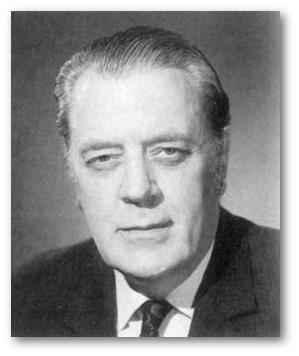
\includegraphics[width=\linewidth]{chapter_4/M_G_Kendall_shadow.png}
\caption{Maurice G. Kendall (6 September 1907 -- 29 March 1983) was a British statistician, widely known for his contribution to statistics. The Kendall tau rank correlation is named after him.}
\end{marginfigure}

\paragraph{Relationship with Kendall's $\tau$.}Some authors (e.g.~\citep{Joachims2002, chen2009unified, wauthier2013efficient}) present the RankSVM model as the model that maximizes a surrogate of the \emph{\gls{Kendall}} correlation coefficient. We will show that maximizing Kedall's $\tau$ and minimizing the pairwise disagreement yield equivalent optimization problems.

Kendall's $\tau$ can be defined as 
$$
\tau = \frac{P - Q}{P + Q}
$$
where $P$ is the number of \emph{concordant pairs}, that is, the number of elements $i > j$ such that $\alpha_i \geq \alpha_j$ and $Q$ is the number of of \emph{discordant pairs}, that is, the number of elements $i > j$ such that $\alpha_i < \alpha_j$. An equivalent formulation of Kendall's $\tau$ is~\citep{Joachims2002}
$$
\tau = 1 - \frac{2 Q}{\binom{n}{2}}
$$


From here it is clear that maximizing the Kendall $\tau$ coefficient is equivalent to minimizing the number of discordant pairs. Since the pairwise disagreement counts the number of discordant pairs, both approaches are equivalent.



%%%%%%%%%%%%%%%%%%%%%%%%%%%%%%%%%%%%%%%%%%%%%%
%%% Results
%%%%%%%%%%%%%%%%%%%%%%%%%%%%%%%%%%%%%%%%%%%%%%
%
\section{Experiments}\label{section:results}


\subsection{Ordinal regression and dimensionality}

The models that we have presented vary greatly in terms of parameters to estimate. Given that $k$ is the number of classes and $p$ is the dimensionality (number of features) of the dataset, the least absolute error and RankLogistic models estimate $p + 1$ parameters, the ordinal logistic model estimates $p + k$ parameters and the multiclass classification model estimates $k \times (p+1)$ parameters. While methods with more parameters can express a richer set of decision functions, the increase in the number of parameters to estimate also induces a higher variance of the estimates which can result in poor generalization performance in settings such as decoding in which the number of samples is very limited and the dimensionality of the dataset is high.

To illustrate this problem we computed the generalization error of the different methods as we increase the dimensionality of a synthetic dataset. The setting is the following: the data is generated by applying a random linear regression model with 10\% of informative nonzero regressors and Gaussian centered noise such that the signal-to-noise ratio is 10:1. The target variable is the discretized in 5 bins such that the number of samples is equal for each class. All models have a squared $\ell_2$ penalization term that has been set chosen among a grid of 10 log-spaced values between $10^{-3}$ and $10^6$  by nested 5-fold cross-validation. The generalization score is computed by 10-fold cross-validation on an equally spaced grid of features between 100 and 600 features. 

\begin{figure}
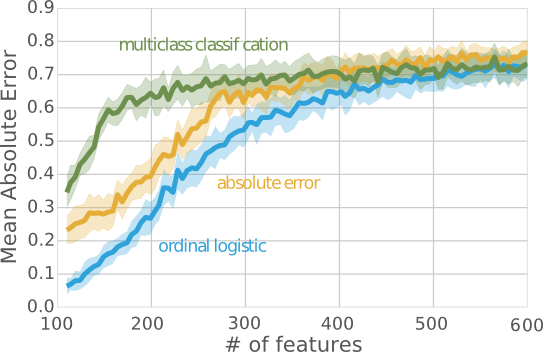
\includegraphics[width=\linewidth]{chapter_4/or_dimension.png}
\caption{Generalization error as the number of dimensions increase on a synthetic dataset (lower is better). In the low sample regime, ordinal logistic regression outperforms the other methods, but as the number of dimension increases the gap between the methods vanishes.
The poor performance of multiclass classification even in the low sample regime can be explained by the model we used to generate the data, which corresponds to the assumptions of ordinal logistic regression.}\label{fig:or_dimension}
\end{figure}


The generalization errors (lower is better) are displayed in Figure~\ref{fig:or_dimension}. It can be observed that in the regime with low number of features, ordinal logistic regression significantly outperforms the other methods, but as the number of dimension increases the gap between the methods vanishes. The data was generated as a discretized linear regression model, which corresponds very closely to the models assumed by the ordinal logistic model\sidenote{in which the prediction function is of the form $\sum_i\mathcal{H}(\theta_i - \B{x}^T \B{w})$}. This might give an advantage to this model and explain the poor behavior of multiclass classification even in the regime with low number of features.




\subsection{Results on two fMRI datasets}


To assess the performance of the different methods presented on the decoding problem, we investigate two fMRI datasets. 

The first dataset that we will considered served as motivation for this chapter. It was presented in \citep{Borghesani2014} and has already been mentioned in Section~\ref{chap2_decoding}. The goal of this experiment is to predict different aspects of the words that subjects were seeing while undergoing an fMRI acquisition. We can consider two different decoding problems based this dataset. As a first step, we investigate the effect of the low level perceptual features characterizing the stimuli: the number of letters composing each word. We will call this decoding problem \emph{length of word}. A second decoding problem that can be investigated on this dataset is to test the relationship between
activation images and the real size of items. In this case, the different stimuli are ordered according to their relative size, i.e. hammer is smaller than cow which is smaller than a whale, etc., so the target variable is of ordinal nature. We will call this decoding problem \emph{size of object}. In both cases we extracted the activation coefficients (beta-maps) using the R1-GLM model with 3hrf basis described in Chapter~\ref{chap:hrf_estimation}. Since we are interested in predicting the target from low level visual features we restrict the decoding problem on an anatomically defined ROI for the primary visual cortex (V1) using the SPM toolbox PickAtlas (13940 voxels). 6 sessions were available for each subject. We trained the model on 5 sessions and evaluated the model on the left out session. We report the average generalization score across subjects.



\begin{marginfigure}[4cm]
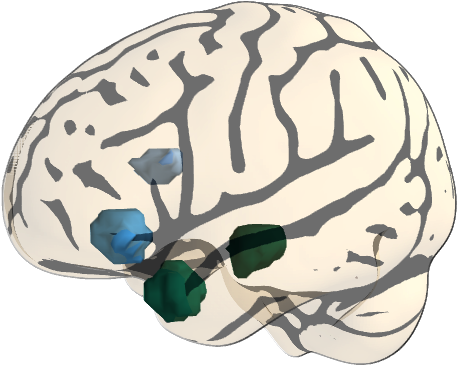
\includegraphics[width=\linewidth]{chapter_4/rois_elo.png}
\caption{Manually labeled ROIs in the \emph{language complexity} dataset~\citep{Cauvet2012thesis}.}\label{fig:rois_elo}
\end{marginfigure}

The second dataset, described
in~\citep{Cauvet2012thesis}, consists of 34 healthy volunteers scanned while
listening to 16 words sentences with five different levels of complexity. These were 1
word constituent phrases (the simplest), 2 words, 4 words, 8 words and 16
words respectively, corresponding to 5 levels of complexity which was
used as class label in our experiments. To clarify, a sentence
with 16 words using 2 words constituents is formed by a series of 8 pairs
of words. Words in each pair have a common meaning but there is meaning
between each pair. A sentence has therefore the highest complexity when all
the 16 words form a meaningful sentence. This dataset contains four manually labeled regions of interest that can be seen in Figure~\ref{fig:rois_elo}: Anterior
Superior Temporal Sulcus, Temporal Pole, Inferior Frontal Gyrus Orbitalis and Inferior Frontal Gyrus triangularis. Further analysis will be limited to these regions of interest. In this dataset each subject only has two sessions, which is insufficient to compute the leave-one session out score. Because of this we instead train the model on 33 subjects and report the cross-validation score on a left-out subject.

\begin{figure*}[t]
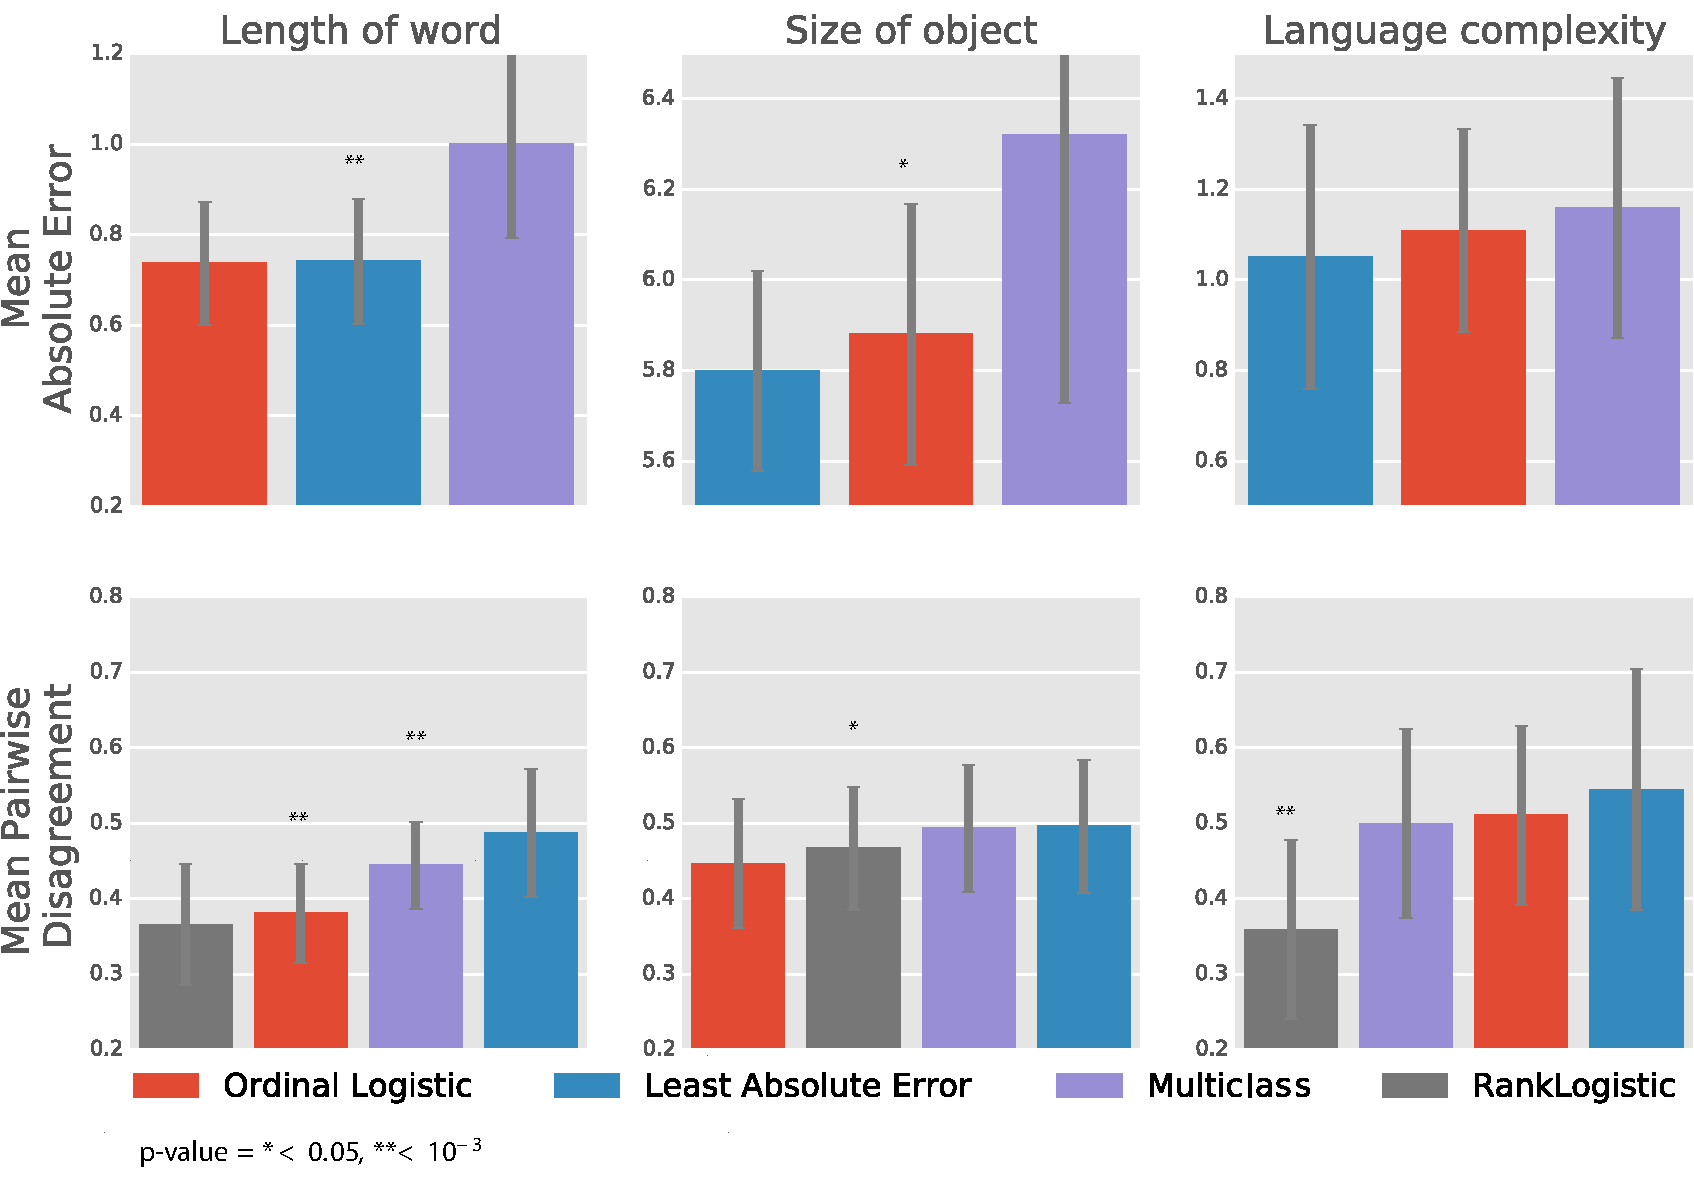
\includegraphics[width=\linewidth]{chapter_4/scores_ordinal.pdf}
\caption[-4cm]{Generalization errors (lower is better) for three fMRI decoding problems. Two different metrics are used corresponding to the rows in the figure: mean absolute error and mean pairwise disagreement. The $*$ symbol represents the $p$-value associated with a Wilcoxon signed-rank test. This test is used to determine whether a given method outperforms significantly the next best-performing method.}\label{fig:scores_ordinal}
\end{figure*}


The generalization errors (lower is better) for these three decoding problems (spanning two datasets) are displayed in Figure~\ref{fig:scores_ordinal}. We considered two different metrics, represented as rows in the figure: mean absolute error and mean pairwise disagreement. We ordered the models by performance and performed a Wilcoxon signed-rank test between each method and the next best performing method to assess whether the difference between both methods is statistically significant. This test is performed by considering the sequence of cross-validation scores obtained for each model. The $p$-value associated with this statistical test is denoted by one or two asterisks, with the convention that $* < 0.05, ** < 10^{-3}$.



When considering the mean absolute error, ordinal logistic regression and least absolute error are the best performing method. The difference between both methods is not significant in any of the three experiments. Multiclass classification is the worst performing method due to the high dimensionality of the problem and the high number of parameters to estimate ($p \times (k-1)$ versus $p + k - 1$ for ordinal logistic).

When considering the pairwise disagreement error, the best performing method is the RankLogistic model. RankLogistic is also the only model that minimizes a surrogate of the evaluation metric.


\section{Discussion}

\newglossaryentry{omnibus}{name={omnibus test},description={Statistical test to asses whether the explained variance in a set of data is significantly greater than the unexplained variance.}}


From the experiments we have examined the relative performance of several classifiers and concluded that ordinal logistic and least absolute error are the best performing methods when evaluated using mean absolute error and RankLogistic is best model when evaluated using mean pairwise disagreement. The superiority of RankLogistic highlights the importance of choosing a model that minimizes a surrogate of the evaluation metric.


A question that arises in practice is: when should the absolute error metric be used and when should the pairwise disagreement metric be used?. The use of one or the other will depend on the particular application in mind. For example, for clinical applications it is often necessary to predict the exact label. If the target variable consists of the different degrees of Alzheimer's disease it is natural to consider an evaluation metric that reflects how close to the true label the prediction is. In this case we would favor the mean absolute error. If however, we are only interested in performing a statistical hypothesis test to claim that the area encodes some information about the stimuli,  then the pairwise disagreement can be considered. 

In this study we have considered the absolute error, but we could have as well considered the squared error loss instead. The linear least squares model, which minimizes a surrogate of this loss, has advantageous computational properties when compared to its absolute error counterpart, the least absolute deviation model: strong convexity, smoothness and analyticity of solutions. However, the use of absolute error resulted in a higher significance when performing hypothesis testing, which is often the end goal of a decoding study. For example, when performing the omnibus test on the ``lenght of word'' decoding problem, we could reject the null hypothesis that the explained variance is not significantly greater than the unexplained variance with a $p$-value < 0.001 when considering the mean absolute error metric and the least absolute error. The $p$-value when considering the mean squared error metric with a linear least squares model (both models have the same number of parameters) was only < 0.005. Similar effects were observed on the other decoding problems.





%



%%%%%%%%%%%%%%%%%%%%%%%%%%%%%%%%%%%%%%%%%%%%%%
%%% Discussion
%%%%%%%%%%%%%%%%%%%%%%%%%%%%%%%%%%%%%%%%%%%%%%
%
\section{Conclusion}
%

In this chapter, we have proposed the usage of two evaluation metrics in the context of brain decoding when the target variable consists of ordered values: the absolute error loss and the pairwise disagreement loss function. We have presented models that optimize a convex surrogate of these loss functions and discussed estimation strategies for these models based on convex optimization. 

We examined the performance of these models on both synthetic and two real world fMRI datasets and identified the best methods for each evaluation metric. Our results show that when considering the absolute error as evaluation metric, the least absolute error and the logistic ordinal model are the best performing methods while when considering the mean pairwise disagreement the RankLogistic was the best performing methods.
For neuroimaging studies, this contribution outlines the best strategies to choose when faced with a decoding problem in which the target variable has a meaningful order.


%
% ---- Bibliography ----
%

\newpage

\begin{fullwidth}
\bibliographystyle{plainnat}
\bibliography{chapter_4/biblio4}
\end{fullwidth}
